\documentclass[11pt]{article}
%\usepackage{cite}
\usepackage[numbers]{natbib}
\usepackage{xcolor}
\usepackage{ulem}
\usepackage{graphicx}
\usepackage{subcaption}
\usepackage{multirow}
\usepackage{booktabs}
\usepackage{amssymb}
\usepackage{tabularx} % in the preamble
\usepackage{algorithm}
\usepackage{algpseudocode}
%\title{\textbf{Draft research question}}
%\author{Mathias Parisot}

      \textwidth 15cm
      \textheight 22cm
      \parindent 10pt
      \oddsidemargin 0.85cm
      \evensidemargin 0.1cm


\begin{document}

\thispagestyle{empty}

\begin{center}

Vrije Universiteit Amsterdam

\vspace{1mm}


\includegraphics[height=28mm]{vu-griffioen-white.pdf}

\vspace{1.5cm}

{\Large Bachelor Thesis}

\vspace*{1.5cm}

\rule{.9\linewidth}{.6pt}\\[0.4cm]
{\huge \bfseries Property Inference Attacks on Neural Networks: Influence of the Architecture\par}
{\huge \bfseries and Implications of the GDPR\par}\vspace{0.4cm}
\rule{.9\linewidth}{.6pt}\\[1.5cm]

\vspace*{2mm}

{\Large
\begin{tabular}{l}
{\bf Author:} ~~Mathias Parisot ~~~~ (2618202)
\end{tabular}
}

\vspace*{1.5cm}

\begin{tabular}{ll}
{\it 1st supervisor:}   & ~~Dr. Dayana Spagnuelo \\
{\it 2nd supervisor:} & ~~Dr. Balazs Pejo \\
{\it 2nd reader:}       & ~~Dr. Michael Cochez
\end{tabular}

\vspace*{2cm}

\textit{A thesis submitted in fulfillment of the requirements for\\ the VU Bachelor of Science degree in Computer Science }

\vspace*{1cm}

\today\\[4cm] % Date

\end{center}

\newpage

\section*{Abstract}

Machine Learning is a set of techniques to train models on tasks such as classification. Classification models are trained to learn and recognize patterns in the training data to categorize it into classes. While the goal of such models is to learn important properties allowing to make correct predictions, there is also a risk that the model learns properties that are unrelated to the classification task. If the training data is sensitive, accessing such properties could lead to privacy leakage. Property Inference Attacks (PIA) are attacks on models aiming at inferring hidden properties of the training set. We focus on PIA on deep neural network classifiers and perform attacks on models trained on face images to infer whether the dataset is balanced. A complex model can solve more difficult classification tasks by learning complex patterns of the data. Because of that, we also investigate whether such models are more sensitive to PIA by studying the influence of the target classifier architecture on the success of the attack. We discuss the implication of our results on data protection laws such as the General Data Protection Regulation\footnote{https://gdpr-info.eu/} (GDPR).

\section{Introduction}

Machine Learning (ML) applications have grown in popularity over the last decade. One of the most common uses of ML is to train models, called classifiers, to learn a mapping function between some input data and a set of classes. A popular way of implementing such models is to use artificial neural networks. Deep Learning (DL) is the field studying neural networks containing several hidden layers. DL models require a large amount of training data and only became popular recently with the advances in hardware and algorithms making it possible to process this data efficiently. Due to the huge amount of data generated by the Internet (communication data, social media websites, pictures, among others), corporations became interested in using ML models to automate some of their decision makings. Because of that, cloud providers such as AWS\footnote{https://aws.amazon.com/machine-learning/}, Microsoft Azure\footnote{https://azure.microsoft.com/en-us/services/machine-learning/}, Google Cloud AI\footnote{https://cloud.google.com/ai-platform} or IBM Watson\footnote{https://www.ibm.com/cloud/machine-learning} started to include ML as a Service to their offer, allowing their users to train and deploy machine learning models given they provide the dataset.\\
With the increasing amount of data generated and its use by companies to gain insights and improve their processes, governments and authorities have been trying to give control to individuals over how their data is used. An example of such action is the legal act in the European Union concerning data protection and privacy called the General Data Protection Regulation. This regulation enforces entities processing personal data to put in place measures to implement principles (see Art. 5) such as:
\begin{itemize}
    \item lawfulness, fairness, and transparency
    \item purpose limitation
    \item data minimization
    \item accuracy
    \item storage limitation
    \item integrity and confidentiality
\end{itemize}
As the training of ML and DL models requires dealing with plenty of data, and because such models are becoming more and more popular, the risk of privacy leakage increases. Because of regulation such as the GDPR, companies processing data need to make sure their datasets stays confidential. However, ML models are sensitive to malicious attacks. Given a classification model, once trained, it can label a data instance to the appropriate class by learning mapping patterns between the training dataset and the set of classes. The mapping is contained within the model parameters, in the case of a neural network, it is the architecture and weight values. Therefore, an attacker knowing the parameters of a trained model, also know some information about the data it was trained on. If the data was composed of personal data, there is a potential confidentiality leak.\\

Attacks on ML models can be classified into four categories. Model extraction \cite{tramer2016stealing, papernot2017practical, wang2018stealing} attacks aim at inferring the behavior of the target model to create a substitute model. A more advanced feat is to create a duplicate by inferring the architecture and the parameter values. Adversarial attacks \cite{goodfellow2014explaining, szegedy2013intriguing} aim at taking advantage of the weaknesses of the classification boundary of the target model to craft data instances that are wrongly classified. Poisoning attacks \cite{mei2015using, jagielski2018manipulating} are similar to adversarial attacks as their goal is to also influence the prediction of the target model, however, they do that by polluting the training set with malicious samples. Model inversion attacks aim at inferring information about the training data, this can be its composition or specific properties of the dataset. 
Depending on the goal of the attacker, we can classify model inversion attacks into three categories. Membership inference attacks \cite{truex2018towards, hitaj2017deep} aim at determining whether a particular data instance was used for training. This creates privacy issues especially when the instance directly maps to an identifiable individual, we can think of a medical records dataset for example. However, such attacks are not always applicable in real-life settings as the attacker needs to get or create a copy of one of the training data beforehand. Property inference attacks \cite{Ateniese2015, Zhang2019, Melis2019} (PIA) aim at reconstructing a representative of a particular class of the training set, or at inferring some hidden properties of the dataset. The first type of PIA is particularly useful when all the instances of a single class represent the same entity. For example, if a model is trained to recognize faces of individuals, the data instances of class A all represent the same individual and it is, therefore, possible to reconstruct an image of this person. While such attacks are particularly impressive for face recognition models, they only build the "average" representation of the class and do not work well if the instances are not similar. The second type of PIA, and the one we are focussing on in this paper, aims at inferring properties learned by the model that are independent of the characteristics of any class, and therefore not related to the main classification task. Such properties can be general statistics about the dataset or can reflect biases in the training set. \\


There have been fewer studies on PIAs: according to \citet{He2019} only 4 papers were published on model inversion attacks against 10 for membership inference attacks. \cite{He2019} also mention that researchers have not yet fully determined the vulnerability of neural network architectures to privacy attacks, PIAs among others. Given the current popularity of computer vision and natural language processing where deep neural networks are the most common model choice, it is reasonable to question to which extend the training datasets are at risk. When training a classifier, the goal is to maximize its performance, usually expressed as its accuracy (ratio of the number of correct classifications to the total number of predictions), recall (true positive rate), and precision (positive predictive value). When the classes are not easily separable, more complex models are required. Because complex models have more parameters and can retain more information about the training set, they usually perform better than less-complex models. Since they retain more information, they could be more sensitive to privacy attacks. In particular, we are interested in the influence of the architecture of a model on its vulnerability to PIAs.\\

\textbf{In case of a trained Neural Network, are sensitive properties of the underlying dataset at risk due to property inference attacks, and if so, how does that risk relate to the architecture of the model?}

\section{Related Works}

\citet{Zhang2019} present a model inversion attack using Generative Adversarial Networks. They study and theoretically prove the relation between a model predictive power and its vulnerability to model inversion attacks. The influence of the predictive power of a model is a hint that more complex models, which should have greater predictive power, should also be more sensitive to model inversion attacks. However, the result of \citet{Zhang2019} was not proven for PIAs. We also focus more specifically on the architecture of the target model.\\
Several studies \cite{Melis2019, Wang2019} performed PIAs in a federated learning \cite{shokri2015privacy} setup which allows multiple clients to train a common model without the need to share data. Only the weights and the gradients after each round of training are exchanged which can help tackle privacy issues. \citet{Melis2019} managed to infer properties that hold for a subset of the training data and that are independent of the property the target model aims at predicting. Because it is performed in a federated learning setting, the attacker has access to the architecture and weights of the model. Moreover, the attack is performed during the training or, at least, requires the model updates that are exchanged between participants. The attack we focus on does not require the gradients' values after each round of training. We also target properties that are true for the whole dataset and not only a subset of it. \citet{Wang2019} propose three kinds of PIAs: class sniffing, quantity inference, and whole determination. Class sniffing detects whether a training label is present within a training round, quantity inference determines how many clients have a given training label in their dataset, whole determination infers the global proportion of a specific label. All of those attacks are extracting properties related to classification labels, and therefore to the main classification task. We focus on properties that are in theory unrelated to the task of the target model.\\
\citet{Geiping2020} study model inversion attacks and analyze the effects of the architecture of the target model on the difficulty of reconstructing input images. They investigate attacks on networks with various widths and depths and found that the width has the greatest influence on the quality of the reconstruction. Their study does not consider PIAs and is restricted to federated learning as they use the gradients' values in their attack.\\
\citet{Ateniese2015} describe the first PIA attack using meta-classifiers, the methodology of the attack we use in our research. Their research is not focussed on the privacy leakage caused by such attack but rather on the impact of the training set properties on the model performance with the commercial benefits that it represents. Moreover, they attack models implemented via Support Vector Machines and Hidden Markov Models using a binary tree meta-classifier but do not experiment with deep neural network models. \citet{Ganju2018} extend the research of \citet{Ateniese2015} to neural networks and notice that a limitation of PIA performance is due to a property of fully connected networks called invariance to weights permutations within the same layer. They propose two successful strategies to reduce the impact of this property: converting a neural network to a canonical form and using a deep set architecture. They use a pre-trained network to generate an embedding which they feed as input to their target neural network. They perform the attack using the weights of the fully connected network following the pre-trained one and do not study the influence of the type of layers and the architecture of the model on the attack performance.\\

\section{Methodology}
To answer the research question, we will perform several PIAs on different target model architectures. For each architecture, we will train attack models and evaluate their performance. This section presents the attack strategy alongside with the assumptions about the target model. \\

\subsection{Threat model}

We suppose the target model is a deep neural network classifier. The training dataset of the classifier contains sensitive data according to the definition used in Article 9.1 of the GDPR. The attack is performed in a white-box setting, which means the attacker has access to the full architecture and parameter values of the model. While a white-box model may be seen as a big assumption in some scenario, it is realistic in ours as it is common in some machine learning paradigms such as Federated Learning \cite{shokri2015privacy} where the clients, and sometimes the server, have full knowledge of the model, and access is only restricted to the dataset. Moreover, model extraction attacks have been done to perform adversarial attacks on deep neural networks in a black-box setting. The attackers managed to create a substitute model with a similar decision boundary as the target model allowing them to achieve larger than 88\% misclassification rates in real-world settings \cite{DBLP:journals/corr/PapernotMGJCS16}. The specificities of a model extraction attack fall out of the scope of this study. In here, we assume the attacker has access to the model architecture and parameter values, independent of how this knowledge was obtained. The goal of the attacker is to infer general information about the training dataset such as the proportion of the training data having a property unrelated to the main classification task of the model.

\subsection{Attack Strategy: Property Inference Attack}
In this subsection, we present the general idea of the attack we used in our experiments. We focus on PIAs which goal is to extract general information about the training dataset of the target model. The information is often presented using a property $P$ which can be true or false. For example, if the dataset used contains images of cars, $P$ could be: \textit{the dataset includes 20\% of images of Ferrari}, or any other brand. We can transform a PIA into a classification task where the goal is as follows: given a trained model, determine whether it was trained using a dataset presenting the given target property $P$. It is then possible to train a classifier to solve the previous classification task. Such a model is called a meta-classifier because the dataset on which it is trained on is composed of models which are themselves classifiers.

The PIA used in this paper is the baseline attack presented in \cite{Ganju2018}. The main idea is to use a meta-classifier to train an attack model $M_a$ which takes as input the weights of a trained model and outputs the probability that the target property $P$ is true for the training set of the input model. Once the attack model is trained, the attacker can give it the target model $M_t$ as input and know whether the property $P$ is true for the dataset used to train the target model. The main problem is then to find enough trained models to use as the training set for the attack model $M_a$. This is solved by using shadow models with the same architecture as the target model $M_t$. The attacker trains $k$ shadow models ($M_{s1}$ ... $M_{sk}$) on k datasets ($D_1$ ... $D_k$ respectively) specifically crafted to contain or not the target property $P$. The general overview of the attack is described in Figure \ref{pia_diagram}.

This PIA is the baseline attack presented in \cite{Ganju2018}. This paper is not focused on the PIA itself but rather on the behavior of the PIA performed on models with different complexities. \\ %We discuss the details of the target models and their complexities in section 2.\\

\begin{figure}[h]
    \centering
    \begin{minipage}{\textwidth}
        \centering
        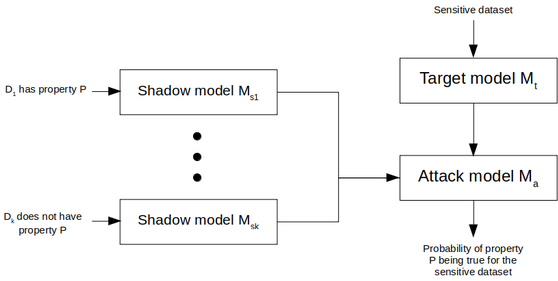
\includegraphics[width=0.99\textwidth]{pia_diagram2.png} % first figure itself
        \caption{Property Inference Attack using a meta-classifier and a dataset of shadow models.}
        \label{pia_diagram}
    \end{minipage}\hfill
\end{figure}

\section{Experimental Setup}

In this section, we describe the experimental settings: the dataset, the architectures of the target and attack models, and the evaluation metrics. The experiments were performed on a laptop with an Intel i7-8750H (2.20GHz) and 8GB RAM. The operating system is Ubuntu 20.04. The training of the shadow models and the attack models were both done using Pytorch and an Nvidia Quadro P600 GPU.\\

\subsection{Datasets}

CelebFaces Attributes (CelebA) \cite{liu2015faceattributes} is a face attributes dataset containing more than 200000 images of more than 10000 celebrities taken from online. The images are labeled using 40 physical attributes such as hair color, smiling, wearing a hat. We use the dataset to train the shadow models $M_s$ to detect whether the person has their mouth open using the \textit{Mouth\_Open} attribute. Although this might seem like an unimportant classification task, in the time of a COVID-19 pandemic, there have been questions about how technology can help the fight against the virus. Some governments are trying to track the persons who have been in contact with a contaminated subject using mobile applications\footnote{https://www.nature.com/articles/d41586-020-01264-1}, in some countries facial masks became compulsory in public places and companies are marketing mask-detection software\footnote{https://www.theverge.com/2020/5/7/21250357/france-masks-public-transport-mandatory-ai-surveillance-camera-software}. Detecting whether someone has their mouth open can be associated with detecting whether someone is wearing a face mask. The property targeted by the attacker is the balance of the gender proportion of the training set using the \textit{Male} attribute. The images are centered and resized to 64 by 64 pixels.\\

\subsection{Shadow Models}
The shadow models are trained to differentiate between images of persons with and without their mouth open.
However, the goal of the attacker is to infer whether the training set of a given model was composed of an unbalanced number of images representing males. The targeted property is a biometric data and is classified as sensitive data according to the GDPR. For a given model, the property $P$ can be formalized as follow: \textit{P is true when the training set of the model is composed of 70\% or more images containing males, otherwise, P is false}. It is important to note that $P$ is not related to the classification task of the model and that the target model does not use, at any time during training, the gender attribute.\\

The shadow models $M_{s_k}$ must have the same architecture as the targeted model, and be trained to a reasonable level of accuracy for the network to retain some information about the training set. For example, all of our shadow models have at least 85\% accuracy on the mouth open classification task when the baseline distribution of the dataset is 51.7\%. For the attack to be effective, a large number of shadow models need to be trained. For each target model architecture, we constructed 1800 unique training sets of 2000 images from CelebA, one for each of the 1800 shadow models. The computational cost of such training is not negligible so we decide to not use all images of \textit{CelebA} in each shadow dataset $D_{s_k}$, but only use 2000 images each randomly selected from the test set of \textit{CelebA}. Out of the 1800 shadow models, 900  were trained on datasets presenting the property $P$ and 900 without. For each dataset, the exact proportion of males was randomly taken from a uniform distribution either above or below 70 respectively.\\

The shadow model architectures are composed of up to 9 layers which can each be of three kinds: convolution layers, pooling layers, fully connected layers. The description of each layer is presented in Table \ref{layer_description}. We trained 9 architectures ($A_1$ to $A_9$) which are presented in Table \ref{shadow_architecture}. The models take as input 64 by 64 RGB face images and output the probability of each picture representing a person with mouth open. All the networks are composed of 1 to 3 convolution layers, each followed by a max-pooling layer with a ReLU activation, and 1 to 3 fully connected layers with a ReLU activation. The shadow models were trained using the Mean Squared Error loss and the Adam optimizer with a learning rate of 0.001 during 50 epochs.\\

\begin{table}[h!]
\centering
\begin{tabular}{@{}ll@{}}
\toprule
Layer              & Description       \\ \midrule
Convolution 1     & 6 filters 5x5     \\
Max-pool          & 2x2, ReLU         \\
Convolution 2     & 16 filters 5x5    \\
Max-pool          & 2x2, ReLU         \\
Convolution 3     & 32 filters 5x5    \\
Max-pool          & 2x2, ReLU         \\
Fully-Connected 1 & 120 neurons, ReLU \\
Fully-Connected 2 & 84 neurons, ReLU  \\
Fully-Connected 3 & 1 neuron          \\ \bottomrule
\end{tabular}
\caption{Description of the different layers used in the shadow architectures.}
\label{layer_description}
\end{table}



\begin{table}[h!]
\centering
\begin{tabular}{@{}lccccccccc@{}}
\toprule
    & Conv 1               & Max-pool             & Conv 2               & Max-pool             & Conv 3               & Max-pool             & FC 1                 & FC 2                 & FC 3                 \\ \midrule
    & \multicolumn{1}{l}{} & \multicolumn{1}{l}{} & \multicolumn{1}{l}{} & \multicolumn{1}{l}{} & \multicolumn{1}{l}{} & \multicolumn{1}{l}{} & \multicolumn{1}{l}{} & \multicolumn{1}{l}{} & \multicolumn{1}{l}{} \\
A 1 & \checkmark           & \checkmark           & \checkmark           & \checkmark           & \checkmark           & \checkmark           & \checkmark           & \checkmark           & \checkmark           \\
A 2 & \checkmark           & \checkmark           & \checkmark           & \checkmark           & \checkmark           & \checkmark           & \checkmark           &                      & \checkmark           \\
A 3 & \checkmark           & \checkmark           & \checkmark           & \checkmark           & \checkmark           & \checkmark           &                      &                      & \checkmark           \\
A 4 & \checkmark           & \checkmark           & \checkmark           & \checkmark           &                      &                      & \checkmark           & \checkmark           & \checkmark           \\
A 5 & \checkmark           & \checkmark           & \checkmark           & \checkmark           &                      &                      & \checkmark           &                      & \checkmark           \\
A 6 & \checkmark           & \checkmark           & \checkmark           & \checkmark           &                      &                      &                      &                      & \checkmark           \\
A 7 & \checkmark           & \checkmark           &                      &                      &                      &                      & \checkmark           & \checkmark           & \checkmark           \\
A 8 & \checkmark           & \checkmark           &                      &                      &                      &                      & \checkmark           &                      & \checkmark           \\
A 9 & \checkmark           & \checkmark           &                      &                      &                      &                      &                      &                      & \checkmark           \\
    & \multicolumn{1}{l}{} & \multicolumn{1}{l}{} & \multicolumn{1}{l}{} & \multicolumn{1}{l}{} & \multicolumn{1}{l}{} & \multicolumn{1}{l}{} & \multicolumn{1}{l}{} & \multicolumn{1}{l}{} & \multicolumn{1}{l}{} \\ \bottomrule
\end{tabular}
\caption{Layer-level description of each shadow architectures. The detailed description of the parameters in each layer is presented in Table \ref{layer_description}.}
\label{shadow_architecture}
\end{table}


\subsection{Attack Model and Evalution}
The attack model classifies shadow models as models trained on a dataset presenting the property $P$ or not. The dataset used is composed of the 1800 shadow models and is split into training (1500 shadow models), validation (100 models), and test sets (200 models). The training algorithm is presented in Algorithm \ref{attack_algo}. The attack model is a deep neural network that was tunned using the validation set and finally evaluated on the test set. The architecture of the model is presented in Table \ref{attack_architecture}. The inputs of the attack model are the flattened weights of the model it is trying to classify as having the property $P$ or not. Therefore, a shadow model architecture with a larger number of parameters induces a wider input layer for the attack model. We created 30 attack models for each shadow model architecture and present the average performance across the 30 repetitions. All the networks are composed of 2 to 4 fully connected layers with ReLU activation. The attack models were trained using the Mean Squared Error loss function and the Adam optimizer with a learning rate of 0.001 during 20 epochs. For each architecture, we compute the accuracy, recall, and precision on the test set containing 200 models.\\

\begin{algorithm}
\caption{Attack model training}\label{attack_algo}
\begin{algorithmic}[1]
\Procedure{Train\_Attack}{$D, n$}
\State{$D$ dataset with images, n number of shadow models to train}
\State $D_{shadow}\gets \{\}$\Comment{The dataset containing shadow models}
\For{$k \gets 1,n$}
\State{$D_{s_k} \gets$ subset of $D$ with or without property $P$}
\State{$S_k \gets train(D_{s_k})$}\Comment{$S_k$ shadow model}
\State{$W_{s_k} \gets getWeights(S_k)$}\Comment{$W_{s_k}$ list of weights of model $S_k$}
\State{$D_{shadow} \gets D_{shadow} \cup \{W_{s_k}$\}}
\EndFor

\State{$A \gets train(D_{shadow})$}\Comment{$S_k$ shadow model}

\State \textbf{return} $A$\Comment{The attack model}
\EndProcedure
\end{algorithmic}
\end{algorithm}

\begin{table}[h!]
\centering
\begin{tabular}{@{}ll@{}}
\toprule
Name              & Description       \\ \midrule
Fully-Connected 1 & 10 neurons, ReLU  \\
Fully-Connected 2 & 10 neurons, ReLU  \\
Fully-Connected 3 & 10 neurons, ReLU  \\
Fully-Connected 4 & 1 neuron          \\ \bottomrule
\end{tabular}
\caption{Architectures of the attack model. FC1 is the input layer and FC4 the output layer.}
\label{attack_architecture}
\end{table}

\section{Results and Discussions}

Figure \ref{accuracy_perf} presents the accuracy of the attacks on each target model architecture. The accuracy of the attack is between 56 and 80\% depending on the architecture, so the target models do retain information that they are not intended to learn. We created as many models presenting the property P as ones not presenting it, therefore, the expected baseline is 50\% accuracy. Most of the architectures have less than 67\% attack accuracy so the actual real-world threat is low. In a real-world setting, the attackers have only one target model to attack, therefore, they must be close to certain (close to 100\% attack accuracy) that the model present the property P. However, we did not spend time tuning the meta-classifier architecture and we believe significant improvement could be made at this level. Moreover, \citet{Ganju2018} have shown that it is possible to significantly increase the accuracy of this attack using representations that are invariant to node permutations. They managed to get almost perfect accuracy making the attack performable in a real-world setting. Whether using such representations on convolutional neural networks results in similar attack accuracies is still to be determined. One of the goals of this study was to establish whether there is a relationship between a model complexity, which we define by its number of parameters, and its sensibility to PIAs, defined as the accuracy of the attack. According to Figure \ref{accuracy_weight}, there does not seem to be a relationship.\\ 

\begin{figure}[h!]
    \centering
    \begin{minipage}{\textwidth}
        \centering
        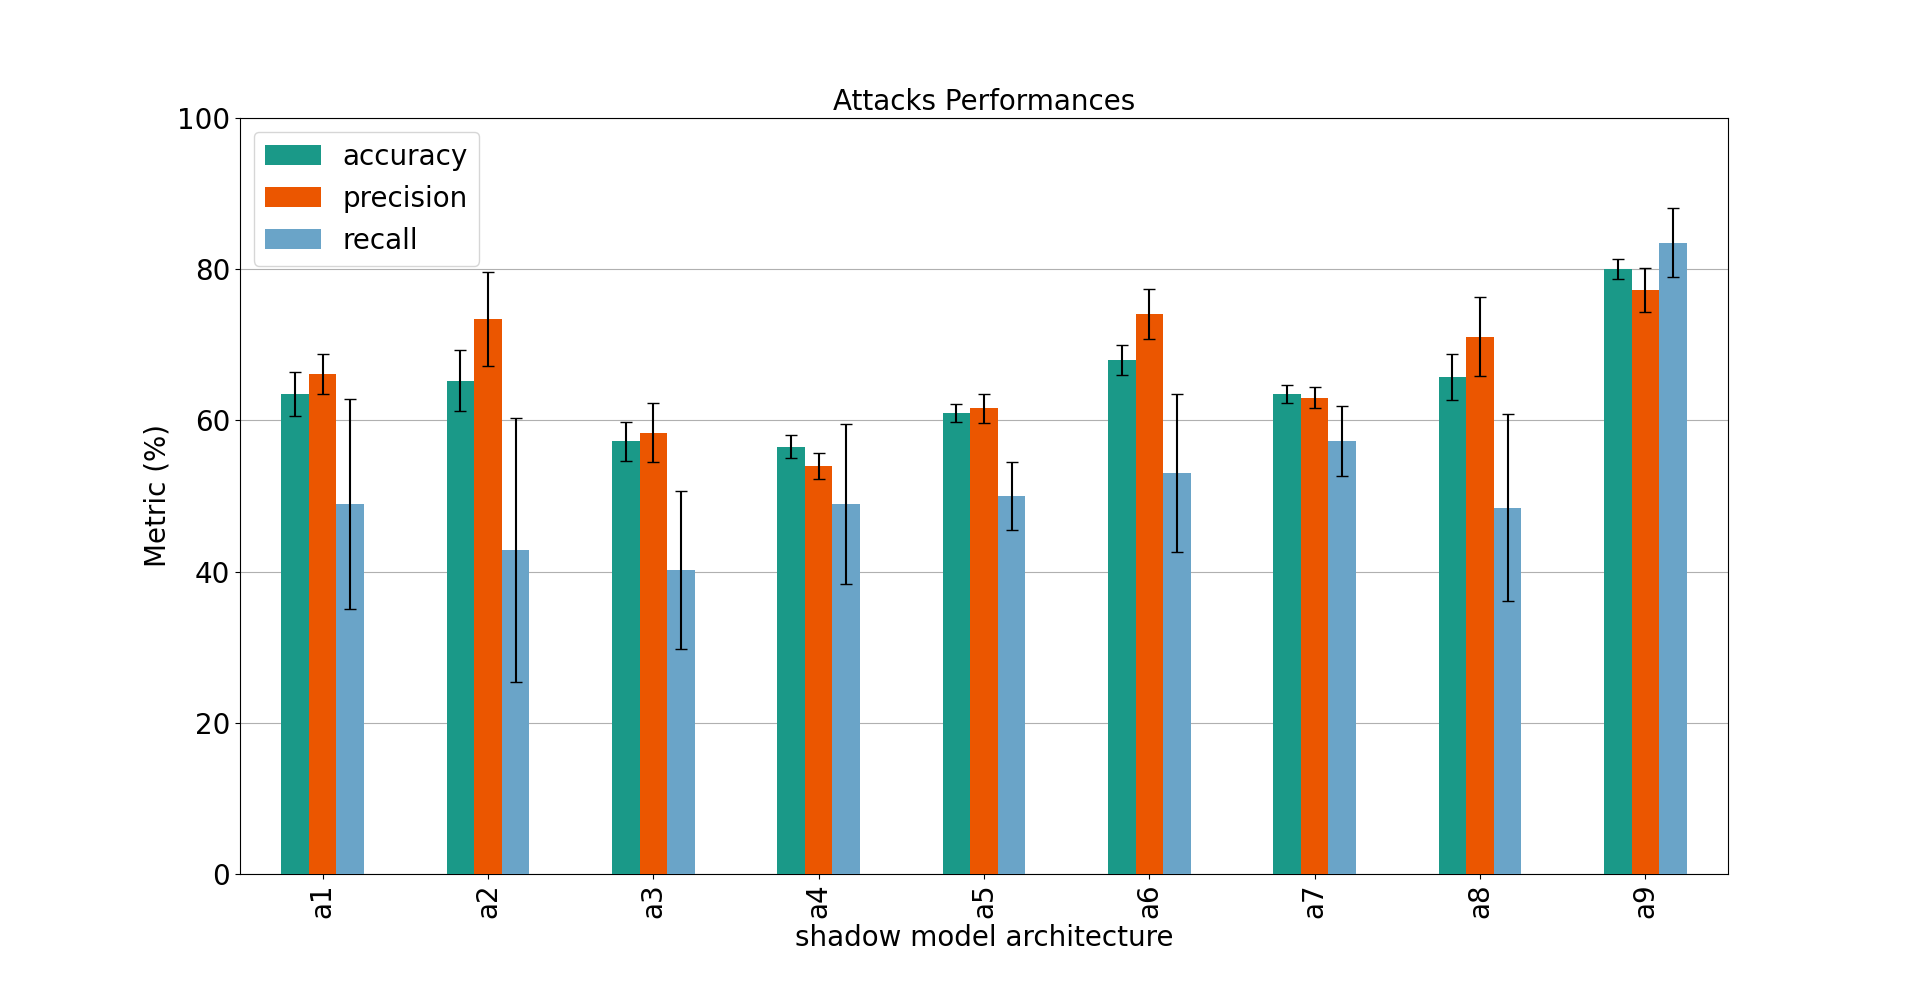
\includegraphics[width=0.99\textwidth]{accuracy_perf.png} % first figure itself
        \caption{Accuracy, precision (positive predictive value), and recall (true positive rate) of the attacks on each architecture. Each bar corresponds to the median of the 30 attacks, and the error bars are $\pm$ the standard deviation.}
        \label{accuracy_perf}
    \end{minipage}\hfill
\end{figure}

\begin{figure}[h!]
    \centering
    \begin{minipage}{\textwidth}
        \centering
        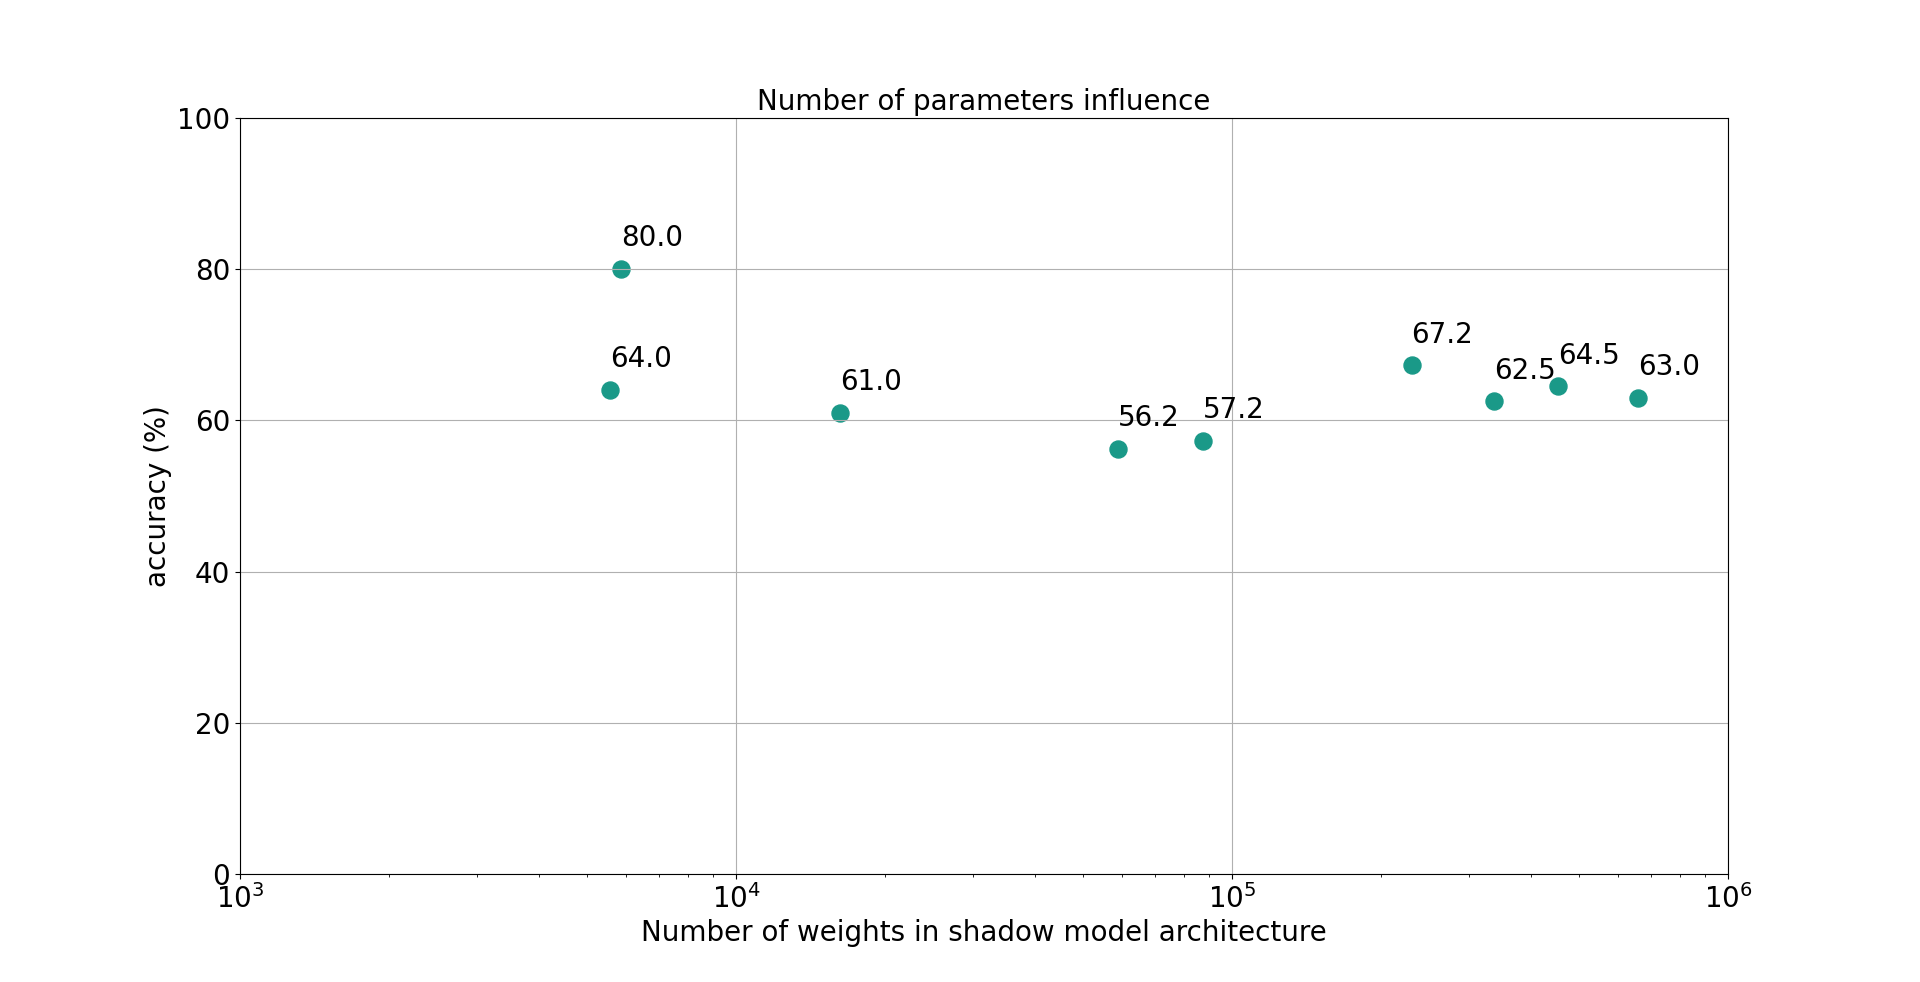
\includegraphics[width=0.99\textwidth]{accuracy_weight.png} % first figure itself
        \caption{Influence of the complexity of the target model (express as the number of parameters) on the accuracy of the attacks on each architecture. Each dot corresponds to the median of the 30 attacks.}
        \label{accuracy_weight}
    \end{minipage}\hfill
\end{figure}

We performed PIAs on distinctive neural network architectures presenting convolution layers. Because convolution layers and fully connected ones play different roles in a convolutional neural network, we studied whether the type of layers used has an impact on the accuracy of the attack. To do that, we conducted three PIAs on each of the architectures presented in Table \ref{shadow_architecture}. The first PIA uses all the weights of the shadow model, the second PIA only uses the weights of the convolution layers, and the third one only the weights of the fully connected layers. Figure \ref{accuracy_conv_fcn} presents the accuracy of the three attacks. For most shadow model architecture, the PIA using only the fully connected weights performs as well, and sometimes better, as the PIA using the weights from both types of layers. The information leaked by a convolutional neural network seems to be contained in the fully connected part of the network.\\

\begin{figure}[h!]
    \centering
    \begin{minipage}{\textwidth}
        \centering
        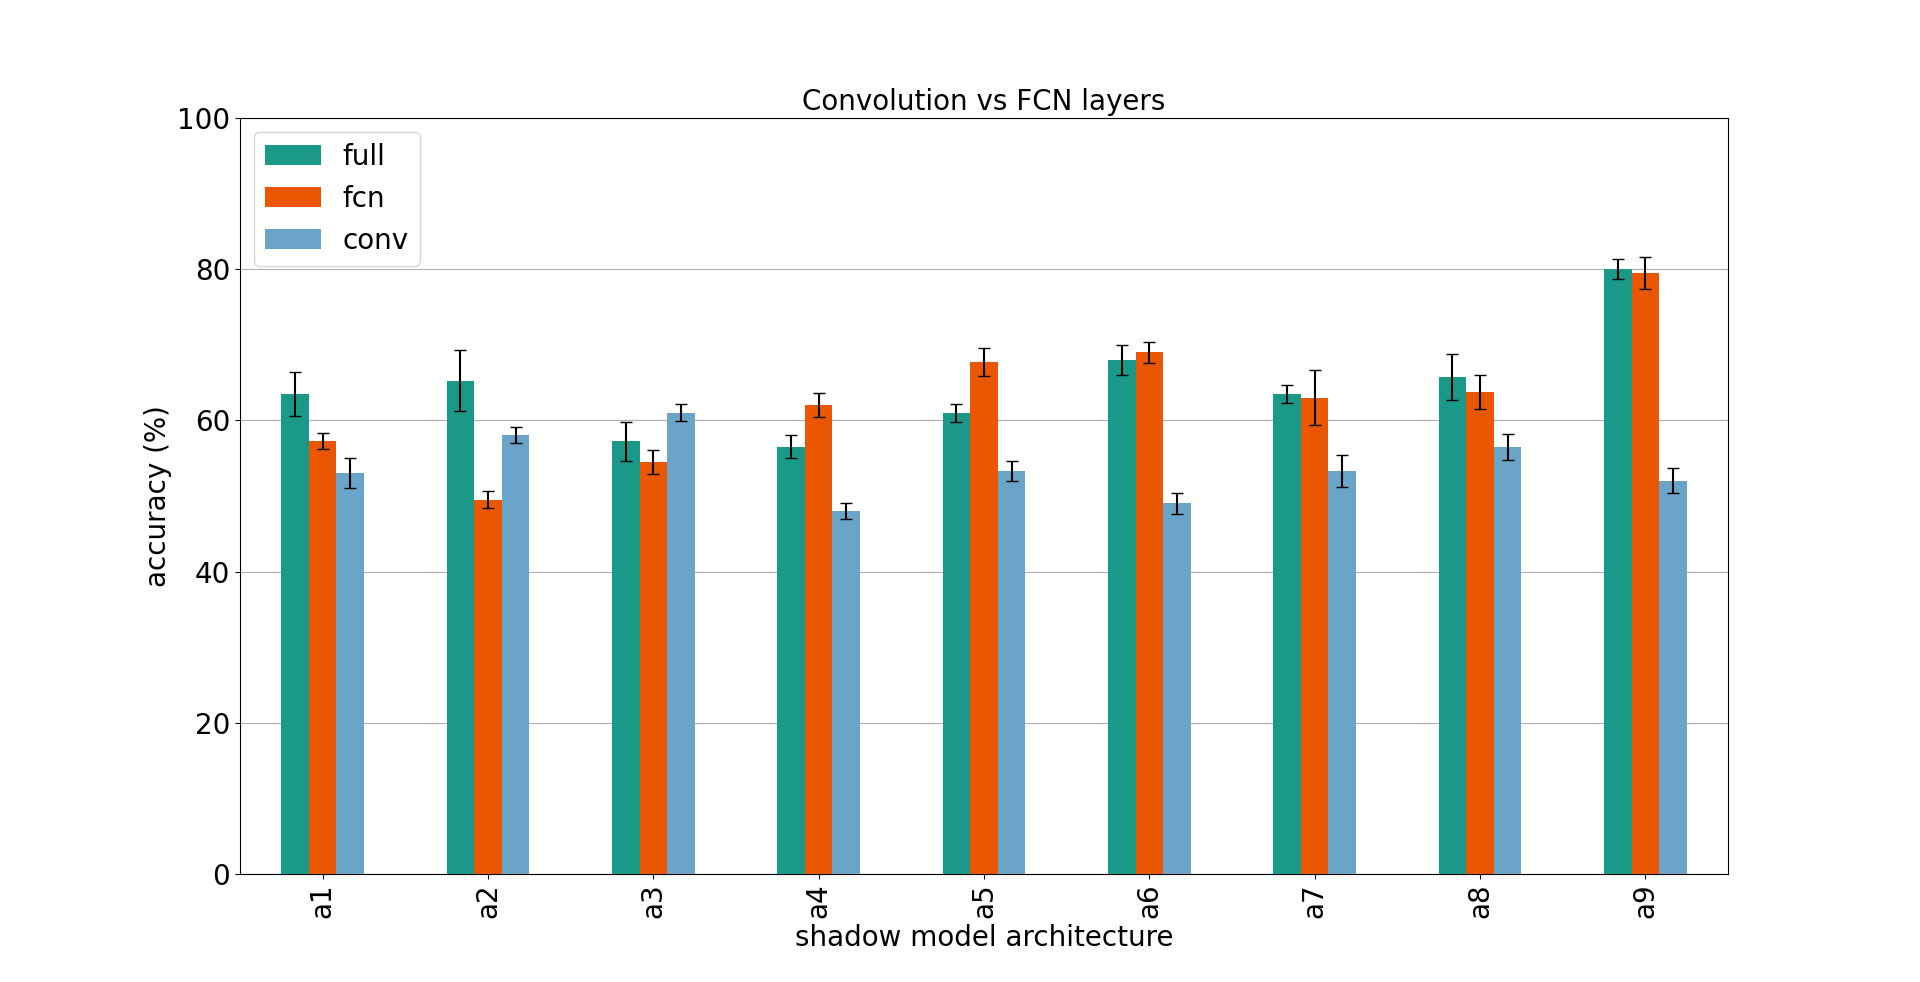
\includegraphics[width=0.99\textwidth]{accuracy_conv_fcn.png} % first figure itself
        \caption{Comparaison of the accuracies of the attacks on each architecture using all the target model weights (full), only the fully connected layers weights (fcn), and only the convolution layers weights (conv). Each bar corresponds to the median of the 30 attacks, and the error bars are $\pm$ the standard deviation.}
        \label{accuracy_conv_fcn}
    \end{minipage}\hfill
\end{figure}


Our goal was to determine if the dataset used to train a CNN model presented a property $P$, in our case whether the dataset was unbalanced. This attack can be performed using other properties $P$ as well. Theoretically, any property $P$ could be inferred from the model as long as the attackers can generate datasets with and without it. We could, for example, infer whether the training set was normalized, or whether it contains a picture of a given person. In that case, when the instances of the same class represent the same entity (same person), a PIA can be transformed into a membership inference attack with the difference that it is not focused on a specific data instance but on whether the whole dataset contains a particular class of image (a particular person). In a real-world setting, this can turn out to be a more important threat. A membership inference attack on portray images risks to fail when the attackers do not possess the exact data instance that is present in the dataset. It is unlikely that the attackers own the same image, however, it is more likely that they possess a dataset of pictures of their target person. They can create shadow datasets with and without pictures of their target, use them to train shadow models, and perform a PIA.\\

Article 5.1 of the GDPR mentions that the processing of personal data shall be limited to what is necessary in relation to the purposes for which they are processed. This property is called data minimization, and it is broken if a data processor shares a model that was trained using personal data. With the PIA discussed, we highlight the surplus of information given to the models and the risk of inference by an attacker. Data processors should consider that information can be extracted from a model and make sure that they train models on data that is only relevant to the classification task. It is the role of data processors to inform users when they give their consent for personal data processing, that there is a risk of privacy leakage.\\

\section{Conclusion}
There is a  risk of leaking general information about the training set when training a neural network. 
In this paper, we further studied a PIA methodology by performing several attacks on different deep neural network architectures. We confirmed that convolutional neural networks are also sensible to PIA, and we emphasized the importance of fully connected layers in the information leakage. We did not observe a relation between the number of weights the target model contains and its sensibility to PIA. Our results stress the dangers of sharing models trained on sensitive dataset and question the usage of federated learning when dealing with personal data.\\

%\clearpage
%\renewcommand\bibliographytypesize{\small}
%\bibliographystyle{alpha}
%\bibliography{references.bib}{}
%\bibliographystyle{unsrtnat}
\bibliographystyle{unsrtnat}
\bibliography{references.bib}


\end{document}
